\documentclass[12pt]{article}
\usepackage[hidelinks]{hyperref}    
\usepackage[all]{hypcap}
\usepackage{amssymb}
\usepackage{amsmath}
\usepackage{graphicx}
\graphicspath{{../images/}}
\title{\textbf{Analisi Matematica\\Funzioni goniometriche}}
\date{04 Ottobre 2024}
\author{Andrea Malvezzi}
\begin{document}
\maketitle
\pagebreak
\tableofcontents
\pagebreak
\section{Circonferenza goniometrica}
La circonferenza goniometrica è una speciale circonferenza, rappresentata dalla seguente equazione:
\begin{equation}
    x^2 + y^2 = 1 \label{eq:circ_goniom}
\end{equation}
Tale circonferenza ha inoltre lunghezza pari a $2\pi$.
\begin{figure}[!htb]
    \centering
    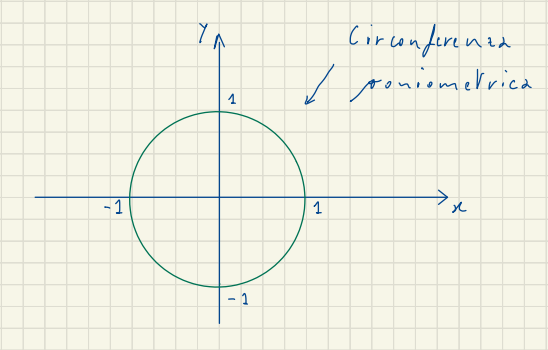
\includegraphics[width=1\textwidth, height=.7\textheight,keepaspectratio]{lezione_6/circonferenza_goniometrica.PNG}
    \begin{center}
        \caption{\label{fig:circ_goniom}La circonferenza goniometrica.}
    \end{center}
\end{figure}
\pagebreak
\subsection{Angoli in gradi e in radianti}
In questa circonferenza si opera basandosi su angoli, che possono essere espressi in \textit{gradi} oppure in \textit{radianti}.
\begin{figure}[!htb]
    \centering
    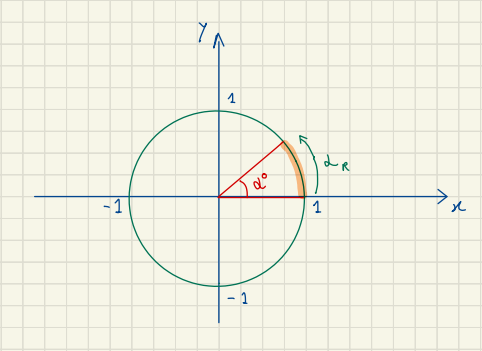
\includegraphics[width=1\textwidth, height=.7\textheight,keepaspectratio]{lezione_6/circonferenza_goniometrica_angolo.PNG}
    \begin{center}
        \caption{\label{fig:angolo_circonferenza}Un angolo $\alpha^{\circ}$ in gradi ed il suo corrispettivo in radianti $\alpha^r$.}
    \end{center}
\end{figure}\\
Per passare da un angolo in gradi ad uno in radianti, si usa la seguente proporzione:
\begin{equation}
    \alpha^{\circ}:360=\alpha^r:2\pi \label{eq:gradi_radianti}
\end{equation}
Che si può semplificare in:
\begin{equation}
    \alpha^r=\alpha^{\circ} \cdot \dfrac{\pi}{180}  \label{eq:gradi_radianti_solved}
\end{equation}
\section{Seno e Coseno sulla circonferenza goniometrica}
Sia $P$ un punto sulla circonferenza goniometrica tale che $P(X_p,Y_p)$.\\
Allora:
\begin{equation}
    \begin{cases}
        P(X_p,Y_p),\\
        \sin{\alpha} = Y_p,\\
        \cos{\alpha} = X_p
        \label{eq:sin_cos_definizione}
    \end{cases}
\end{equation}
Che rappresentato sulla circonferenza goniometrica diventa:
\begin{figure}[!htb]
    \centering
    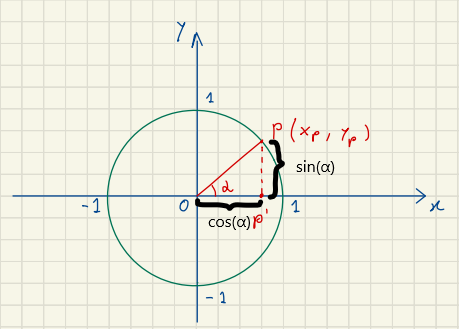
\includegraphics[width=1\textwidth, height=.7\textheight,keepaspectratio]{lezione_6/sin_cos_definizione.png}
    \begin{center}
        \caption{\label{fig:sin_cos_definizione}Il seno ed il coseno corrispondono ai due cateti di un triangolo rettangolo.}
    \end{center}
\end{figure}
\pagebreak
\subsection{Funzioni dispari e pari}
Inoltre, come facilmente osservabile sulla circonferenza goniometrica, invertendo il segno del parametro del coseno, si ottiene sempre lo stesso risultato, mentre invertendo quello del parametro del seno si ottiene un risultato a segno inverso.\\
Questo perché il coseno è una funzione \textbf{pari}, mentre il seno è \textbf{dispari}.
\begin{figure}[!htb]
    \centering
    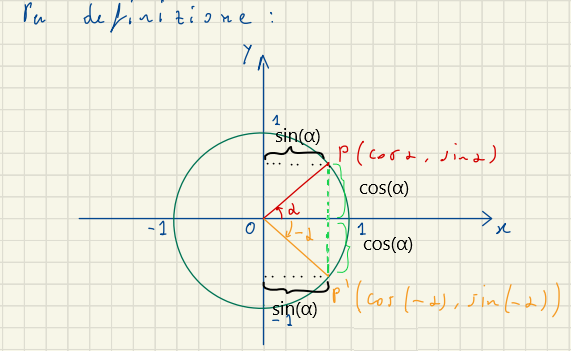
\includegraphics[width=1\textwidth, height=.7\textheight,keepaspectratio]{lezione_6/sin_cos_dispari_pari.PNG}
    \begin{center}
        \caption{\label{fig:sin_cos_dispari_pari}Esempio di parità del coseno e di disparità del coseno.}
    \end{center}
\end{figure}
\section{Funzione Tangente}
\end{document}